\section{Background}

\subsection{Intel SGX: A TEE Implementation}

Intel SGX~\cite{sgxdoc} is a popular implementation of TEE. It runs code inside a special ``Enclave'' so that the execution of the code is deterministic, i.e., not affected by other processes or underlying operating system, and the intermediate states is not leaked. In a properly set up system, Intel SGX can defend the attacks from the OS layer and hardware layer.

\begin{figure}
    \centering \footnotesize
    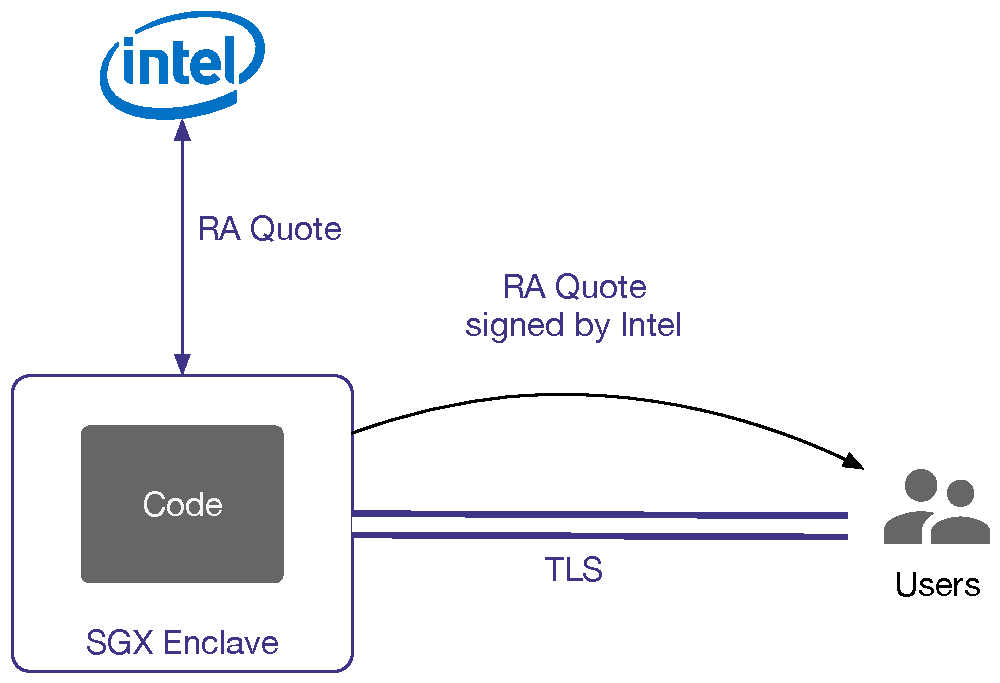
\includegraphics[width=.7\columnwidth]{img/pLIBRA-sgxra}
    \caption{Intel SGX remote attestation procedure.}
    \label{fig:sgx-ra}
\end{figure}

To ensure the execution is finished as expected inside an enclave, a proof can be generated according to a protocol called \textbf{Remote Attestation}. The hardware can generate an \textit{attestation quote} based on the details of hardware, firmware, the code being executed inside the enclave, and other user-defined data produced by the code. The quote is signed by the trusted hardware with credentials embedded during the production process.

Next, the generated attestation quote is sent to the Intel Remote Attestation Service. Intel will sign the quote iff the signing credentials are valid. As each credential is uniquely bound to an Intel CPU unit, fake attestation quotes will never pass the Remote Attestation Service check.

Finally, the attestation quote signed by Intel serves as the proof of a successful execution. It proves that specific code has been run inside an SGX enclave and produces certain output, which implies the confidentiality and the correctness of the execution. The proof can be published and validated by anyone with generic hardware.

Intel SGX and the Remote Attestation protocol is the foundation of confidential contract. Except for Intel SGX, there are also alternative implementation choices like AMD SEV~\cite{amdsev} and ARM TrustZone~\cite{armtrustzone}.

\subsection{Event Sourcing and CQRS}

Event Sourcing is a software design pattern. Instead of storing the latest state of the data, the events causing state transition are recorded in an append-only log. The events are timestamped and can be replayed to reconstruct the state of any time. Since the events are timestamped, the state of the system is deterministic. Command Query Responsibility Segregation (CQRS) is a design pattern by which the read operations and write operations are handled separately. In a CQRS and Event Sourcing combined system, the write operations are recorded as the events and the read operations can be served by the current view of the state. This pattern make a system easy to scale up and avoid conflicts.

For native CPU performance and better security, each confidential contract is bound to only a single or a small set of TEEs as the executor. By this design, the contract state is isolated from each other without consistency guarantee. It becomes a trouble for cross-contract and even cross-chain interoperability.

While it's hard to keep a strong consistency over the states, contracts can still communicate by passing messages to each other on the premise that state transition is still deterministic. In an Event Sourcing / CQRS design, the commands can be initiated from users or contracts and are timestamped on the blockchain strictly. It guarantees the global state is deterministic and therefore enables message passing between contracts. Message passing is a primitive to implement higher level interoperability like contract invocation and token transferring. The read-only operations are not timestamped for better performance.
